\documentclass[letterpaper,11pt]{article}
\oddsidemargin -1.0cm \textwidth 17.5cm

\usepackage[utf8]{inputenc}
\usepackage[activeacute,spanish, es-lcroman]{babel}
\decimalpoint
\usepackage{amsfonts,setspace}
\usepackage{amsmath}
\usepackage{amssymb, amsmath, amsthm}
\usepackage{comment}
\usepackage{float}
\usepackage{amssymb}
\usepackage{dsfont}
\usepackage{anysize}
\usepackage{multicol}
\usepackage{enumerate}
\usepackage{graphicx}
\usepackage[left=1.5cm,top=2cm,right=1.5cm, bottom=1.7cm]{geometry}
\setlength\headheight{1.5em} 
\usepackage{fancyhdr}
\usepackage{multicol}
\usepackage{hyperref}
\usepackage{wrapfig}
\usepackage{subcaption}
\usepackage{siunitx}
\usepackage{cancel}
\usepackage{mdwlist}
\pagestyle{fancy}
\fancyhf{}
\renewcommand{\labelenumi}{\normalsize\bfseries P\arabic{enumi}.}
\renewcommand{\labelenumii}{\normalsize\bfseries (\alph{enumii})}
\renewcommand{\labelenumiii}{\normalsize\bfseries \roman{enumiii})}


\begin{document}

\fancyhead[L]{\itshape{Facultad de Ciencias F\'isicas y Matem\'aticas}}
\fancyhead[R]{\itshape{Universidad de Chile}}

\begin{minipage}{11.5cm}
    \begin{flushleft}
        \hspace*{-0.6cm}\textbf{FI1000-6 Introducción a la Física Clásica}\\
        \hspace*{-0.6cm}\textbf{Profesora:} Paulina Lira\\
        \hspace*{-0.6cm}\textbf{Auxiliares:} Juan Cristóbal Castro \& Alejandro Silva\\
        \hspace*{-0.6cm}\textbf{Ayudantes:} Francisca Bórquez, Catalina Molina \& Erick Pérez\\
        
    \end{flushleft}
\end{minipage}

\begin{picture}(2,3)
    \put(366, 10){
\includegraphics[scale=0.9]{2020-1/Imágenes/logo/dfi-fcfm.pdf}}
\end{picture}

\begin{center}
	\LARGE\textbf{Aux Extra}\\
	\Large{Salvando el C1}
\end{center}

\vspace{-1cm}
\begin{enumerate}\setlength{\itemsep}{0.4cm}

\rfoot[]{pág. \thepage}

\item[]

\item N partículas ubicadas a diferentes alturas $h_1, h_2, . . . h_n$ sobre el eje y son lanzadas simultáneamente, con la misma velocidad $V_{0x}=V_0=cte$, en la dirección positiva del eje x. Por acción de la fuerza de gravedad terrestre las partículas aterrizan en diferentes puntos sobre el eje x.
\begin{figure}[h!]
    \centering
    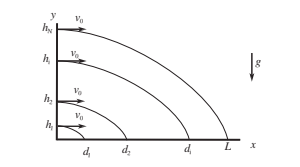
\includegraphics[scale=0.4]{2021-1/Imagenes/Aux extra/Captura de Pantalla 2021-05-04 a la(s) 16.54.42.png}
\end{figure}

\begin{enumerate}
    \item Encuentre la alturas $h_i$ en función del  índice i y los datos del problema para que los puntos donde aterrizan las partículas di estén uniformemente distribuidos entre 0 y L, i.e., que la distancia entre el origen y el primer punto de aterrizaje y las distancias entre dos puntos seguidos cualesquiera, sea constante e igual para todos ellos.
    \item Con qué retardo habría que lanzar las diferentes partículas para que aterrizaran simultáneamente, conservando una distribución uniforme sobre el eje x?
\end{enumerate}

\item Una bloque de masa m está puesto en un aro, de forma circular de radio R, el cual gira en torno al eje vertical como se indica en la figura. Considerando que no existe roce entre el aro y el bloque. Determinar el periodo de rotación del aro
para que el bloque se mantenga en una posición tal que forme un ángulo $\theta$ con la vertical.
\begin{figure}[h!]
    \centering
    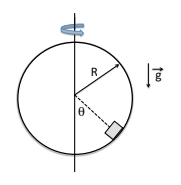
\includegraphics[scale=0.4]{2021-1/Imagenes/Aux extra/Captura de Pantalla 2021-05-04 a la(s) 16.49.26.png}
\end{figure}

\item (Apunte Hugo Arellano, Ejercicio 8) Una linterna asciende verticalmente con rapidez constante $u$ iluminando de forma cónica un área circular sobre el piso. Al mismo tiempo un razón sale de su casa en un trayecto rectilíneo que atraviesa diametralmente el área iluminada. Inicialmente el ratón sale de su casa y la linterna comienza a subir desde el piso a una distancia D del ratón. El cono de iluminación está caracterizado por un 
ángulo directriz $\phi$. Calcule el lapso que el ratón es iluminado por la linterna.

\item Un ciclista pedalea a una frecuencia f. Si el radio del disco es D, el del piñón es P y el de la rueda es R.
 \begin{enumerate}
     \item Determine la velocidad a la que avanza el ciclista.
     \item Debido a una bajada la velocidad del ciclista es el triple de la velocidad anterior. Encuentre su nueva frecuencia.
 \end{enumerate}
\end{enumerate}
\end{document}